\section{Differential Cross-Section}
\label{sec:differential cross-section}

The analysis method is very similar to the previously published one \cite{8tev-90m}. Section~\ref{sec:event analysis} covers all aspects related to the reconstruction of a single event. Section~\ref{sec:diff cs} describes the steps of transforming a raw $t$-distribution into the differential cross-section. The $t$-distributions for the two diagonals are analysed separately. After comparison (Section~\ref{sec:cross checks}) they are finally merged (Section~\ref{sec:final data merging}).

%----------------------------------------------------------------------------------------------------
\subsection{Event Analysis}
\label{sec:event analysis}

The event kinematics are determined from the coordinates of track hits in the RPs after proper alignment (see Sec.~\ref{sec:alignment}) using the LHC optics (see Sec.~\ref{sec:optics}).

%------------------------------

\subsubsection{Kinematics Reconstruction}
\label{sec:kinematics}

For each event candidate 
the scattering angles and vertex positions of both protons (one per arm) are first determined separately by inverting the proton transport equation~(\ref{eq:prot trans}), assuming $\xi = 0$:
\begin{equation}
\label{eq:kin 1a}
	\theta_x^{*\rm L,R} = {v_x^{\rm N} x^{\rm F} - v_x^{\rm F} x^{\rm N}\over v_x^{\rm N} L_x^{\rm F} - v_x^{\rm F} L_x^{\rm N}}\ ,\qquad
	\theta_y^{*\rm L,R} = {1\over 2} \left( {y^{\rm N}\over L_y^{\rm N}} + {y^{\rm F}\over L_y^{\rm F}} \right)\ ,\qquad
	x^{*\rm L,R} = {L_x^{\rm N} x^{\rm F} - L_x^{\rm F} x^{\rm N}\over L_x^{\rm N} v_x^{\rm F} - L_x^{\rm F} v_x^{\rm N}}\ , 
\end{equation}
where the N and F superscripts refer to the near and far units, L and R to the left and right arm, respectively. 
%The formulae optimise the robustness against optics imperfections:
This one-arm reconstruction is used for tagging elastic events, where the left and right arm protons are compared.

Once a proton pair has been selected, all four RPs are used to reconstruct the kinematics of the event, optimising the angular resolution (see Section \ref{sec:resolution}):
\begin{equation}
\label{eq:kin 2a}
		\theta_x^* = {
				\sum {v_x^i}^2 \sum L_x^i x^i - \sum L_x^i v_x^i \sum v_x^i x^i
				\over
				\sum {v_x^i}^2 \sum {L_x^i}^2 - \sum L_x^i v_x^i \sum v_x^i L_x^i
			}\ ,\qquad
		\theta_y^* = {1\over 4} \sum {y^i\over L_y^i}\ ,
\end{equation}
where the sums run over the superscript $i$ representing the four RPs of a diagonal.

Eventually, the scattering angle, $\theta^*$, and the four-momentum transfer squared, $t$, are calculated:

\begin{equation}
\label{eq:th t}
\theta^* = \sqrt{{\theta_x^*}^2 + {\theta_y^*}^2}\ ,\qquad t = - p^2 ({\theta_x^*}^2 + {\theta_y^*}^2)\ ,
\end{equation}
where $p$ denotes the beam momentum.


%------------------------------

\subsubsection{Alignment}
\label{sec:alignment}

TOTEM's usual three-stage procedure~\cite{totem-ijmp} for correcting the detector positions and rotation angles  
has been applied: a beam-based alignment prior to the run followed by two offline methods. First, track-based alignment for relative positions among RPs, and second, alignment with elastic events for absolute position with respect to the beam -- repeated in 15 minutes time intervals to check for possible beam movements.

The offline procedure has been extended further to improve the vertical alignment. The new steps exploit the fact that elastic events with their two collinear protons relate the alignments in the left and right arm with an uncertainty of $20\un{\mu m}$. Furthermore, the horizontal RPs in the right arm recorded a hit distribution usable for vertical alignment in addition to the standard technique based on the vertical RPs, see Figure~\ref{fig:align meth}.

\begin{figure}
\begin{center}
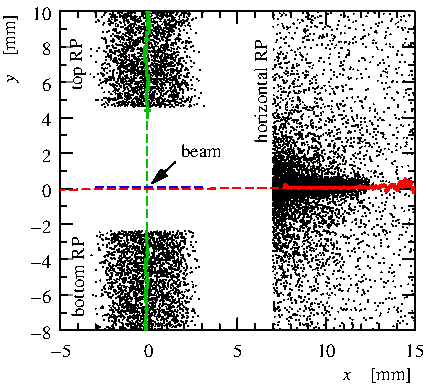
\includegraphics{fig/alignment_method.pdf}
\caption{%
Hit scatter plot in the right-far unit, corresponding to a period of 15 minutes. The black dots represent track hits in the vertical and horizontal RPs. Track hits close to the sensor edges are removed because of possible bias due to acceptance effects.
The green histogram shows the horizontal profile of hits in the vertical RPs, the dashed green line interpolates the profiles between the top and bottom RPs. Similarly, the red histogram gives the vertical profile of the hits in the horizontal RP and the dashed red line its extrapolation to the beam region. The blue dashed line indicates the vertical centre of symmetry of the hits in the vertical RPs (see \cite{totem-ijmp} for more details). The crossing of the dashed lines represents the position the beam centre (the two vertical-alignment results are averaged).
}
\label{fig:align meth}
\end{center}
\end{figure}

Exploiting all the methods, the alignment uncertainties have been estimated to $30\un{\mu m}$ (horizontal shift), $70\un{\mu m}$ (vertical shift) and $2\un{m rad}$ (rotation about the beam axis). Propagating them through Eq.~(\ref{eq:kin 2a}) to reconstructed scattering angles yields $0.28\un{\mu rad}$ ($0.19\un{\mu rad}$) for the horizontal (vertical) angle. RP rotations induce a bias in the reconstructed horizontal scattering angle:
\begin{equation}
\label{eq:alig rot bias}
	\theta_x^* \rightarrow \theta_x^* + c \theta_y^*\ ,
\end{equation}
where the proportionality constant $c$ has a mean of 0 and a standard deviation of $0.005$.


%------------------------------

\subsubsection{Optics}
\label{sec:optics}
It is crucial to know with high precision the LHC beam optics between IP5 and the RPs, i.e. the behaviour of the spectrometer composed of the various magnetic elements.
The optics calibration has been applied as described in~\cite{totem-optics}. This method uses RP observables to determine fine corrections to the optical functions presented in Eq.~(\ref{eq:prot trans}).

The residual errors induce a bias in the reconstructed scattering angles:
\begin{equation}
\label{eq:opt bias}
	\theta_x^* \rightarrow (1 + d_x)\, \theta_x^*\ ,\qquad
	\theta_y^* \rightarrow (1 + d_y)\, \theta_y^*\ .
\end{equation}
For the two-arm reconstruction, Eq.~(\ref{eq:kin 2a}), the biases $d_x$ and $d_y$ have uncertainties of $0.34\un{\%}$ and $0.25\un{\%}$, respectively, and a correlation factor of $-0.89$. These estimates include the effects of magnet harmonics. To evaluate the impact on the $t$-distribution, it is convenient to decompose the correlated biases $d_x$ and $d_y$ into eigenvectors of the covariance matrix:
\begin{equation}
\label{eq:opt bias modes}
\begin{pmatrix} d_x\cr d_y \end{pmatrix} =
	\eta_1 \underbrace{\begin{pmatrix} +0.338\un{\%} \cr -0.234\un{\%} \end{pmatrix}}_{\rm mode\ 1}
	\ +\ \eta_2 \underbrace{\begin{pmatrix} -0.053\un{\%} \cr -0.076\un{\%} \end{pmatrix}}_{\rm mode\ 2}
\end{equation}
normalised such that the factors $\eta_{1,2}$ have unit variance.

%	mode 0			mode 1
%	3.382E-03		-5.278E-04
%	-2.343E-03		-7.618E-04

%------------------------------

\subsubsection{Resolution}
\label{sec:resolution}

Statistical fluctuations in $\theta_y^*$ are mostly due to the beam divergence and can be studied by comparing the angles reconstructed from the left and right arm. As illustrated in Figure~\ref{fig:beam div vert}, the distributions show only minimal deviations from a Gaussian shape.
%
By dividing their standard deviation by a factor of 2, one can estimate the resolution of the two-arm reconstruction (Eq.~(\ref{eq:kin 2a})) of elastic events, see Figure~\ref{fig:resol final}, right.
%
Moreover, measurements of beam emittances \cite{op-elog} indicate that the vertical divergences of the two beams can be considered as equal with a tolerance of about $25\un{\%}$. Exploiting this fact, one can de-convolute the distribution of $\theta_y^{*\rm R} - \theta_y^{*\rm L}$ in order to obtain the beam-divergence distribution, used for the acceptance corrections discussed in Section~\ref{sec:acc corr}.

\begin{figure}
\begin{center}
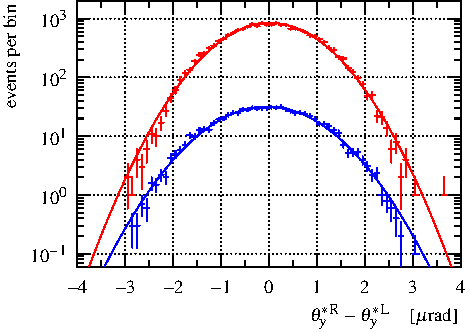
\includegraphics{fig/beam_divergence_fits.pdf}
\caption{%
Difference between vertical scattering angles reconstructed in the right and left arm, for the diagonal 45 top - 56 bottom. Red: data from run start ($0$ to $1\un{h}$ from the beginning of the run). Blue: data from run end ($7$ to $8\un{h}$), scaled by $0.1$. The solid lines represent Gaussian fits.
}
\label{fig:beam div vert}
\end{center}
\end{figure}

In the horizontal projection, a more complex procedure is used since the one-arm reconstruction, Eq.~(\ref{eq:kin 1a}), is strongly influenced by the detector resolution. First, the horizontal beam divergence is estimated from the standard deviation of reconstructed vertices, $\sigma(x^*)$:
\begin{equation}
\label{eq:beam div from vertex}
\sigma^{\rm bd}(\theta_x^*) = {\sigma(x^*) \sqrt 2\over \beta^*}\ .
\end{equation}
It increases from $0.75$ to $0.9\un{\mu rad}$ over the time of the fill. Subtracting this component from the standard deviation of $\theta_x^{*\rm R} - \theta_x^{*\rm L}$, one determines the (mean) spatial resolution of the sensors in each diagonal: $10.7\un{\mu m}$ (45 top -- 56 bottom) and $12.1\un{\mu m}$ (45 bottom -- 56 top). These results have been verified to be time independent. Finally, the beam divergence and sensor resolution components can be propagated through Eq.~({\ref{eq:kin 2a}}) to estimate the $\theta_x^*$ resolution for elastic events, as plotted in Figure~\ref{fig:resol final}, left.


\begin{figure}
\begin{center}
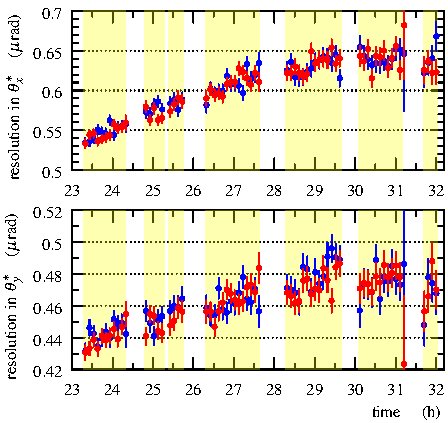
\includegraphics{fig/resolutions_vs_time.pdf}
\caption{%
Angular resolution for the two-arm reconstruction, Eq.~(\ref{eq:kin 2a}), as a function of time (from the beginning of the run). The blue (red) dots correspond to the diagonal 45 bottom -- 56 top (45 top -- 56 bottom). The yellow bands indicate regions of uninterrupted data-taking, whereas in the remaining periods the beam cleaning procedure described in Section~\ref{sec:data taking} was performed.
}
\label{fig:resol final}
\end{center}
\end{figure}

%----------------------------------------------------------------------------------------------------
\subsection{Differential Cross-Section Reconstruction}
\label{sec:diff cs}

For a given $t$ bin, the differential cross-section is evaluated by selecting and counting elastic events:
\begin{equation}
{\d\sigma\over \d t}(\hbox{bin}) =
	{\cal N}\, {\cal U}({\rm bin})\, {\cal B}\, {1\over \Delta t}
	\sum\limits_{t\, \in\, {\rm bin}} {\cal A}(\theta^*, \theta_y^*)\ {\cal E}(\theta_y^*)
	\ ,
\end{equation}
where $\Delta t$ is the width of the bin, ${\cal N}$ is a normalisation factor and the other symbols stand for various correction factors:
 ${\cal U}$ for unfolding of resolution effects, ${\cal B}$ for background subtraction, ${\cal A}$ for acceptance correction and ${\cal E}$ for detection and reconstruction efficiency.

%-------------------------

\subsubsection{Event Tagging}
\label{sec:tagging}

\begin{table}
\caption{The elastic selection cuts. The superscripts R and L refer to the right and left arm. The $\alpha \theta_x^*$ term in cut 3 absorbs the effects of residual optics imperfections, $\alpha$ is of the order of $0.1\un{\mu m/\mu rad}$. The right-most column gives a typical RMS of the cut distribution.
}
\label{tab:cuts}
\begin{center}
\vskip-3mm
\begin{tabular}{ccc}\hline\hline
number & cut & RMS ($\equiv 1\sigma$)\cr\hline
1 & $\theta_x^{*\rm R} - \theta_x^{*\rm L}$				& $3.9\un{\mu rad}$	\cr
2 & $\theta_y^{*\rm R} - \theta_y^{*\rm L}$				& $1.0\un{\mu rad}$	\cr
3 & $x^{*\rm R} - x^{*\rm L} - \alpha \theta_x^*$		& $250\un{\mu m}$ 	\cr\hline\hline
\end{tabular}
\end{center}
\end{table}

The cuts used to select the elastic events are summarised in Table~\ref{tab:cuts}. Cuts 1 and 2 require the reconstructed-track collinearity between the left and right arm. Cut 3 ensures that the protons come from the same vertex (horizontally). The correlation plots corresponding to these cuts are shown in Figure~\ref{fig:cuts}. Thanks to the very low beam divergence, the collinearity cuts are very powerful, and consequently other conceivable cuts (cf. Table~2 in~\cite{epl101-el}) bring no significant improvement.

Since a Monte-Carlo study shows that applying the three cuts at the $3\un{\sigma}$ level would lead to a loss of about $0.5\un{\%}$ of the elastic events, the cut threshold is set to $4\un{\sigma}$.

The tagging efficiency has been studied by applying the cuts also at the $5\un{\sigma}$-level. This selection has yielded $0.3\un{\%}$ more events in every $|t|$-bin. This kind of inefficiency only contributes to a global scale factor, which is irrelevant for this analysis because the normalisation is taken from a different data set (cf. Section~\ref{sec:normalisation}).


\begin{figure}
\begin{center}
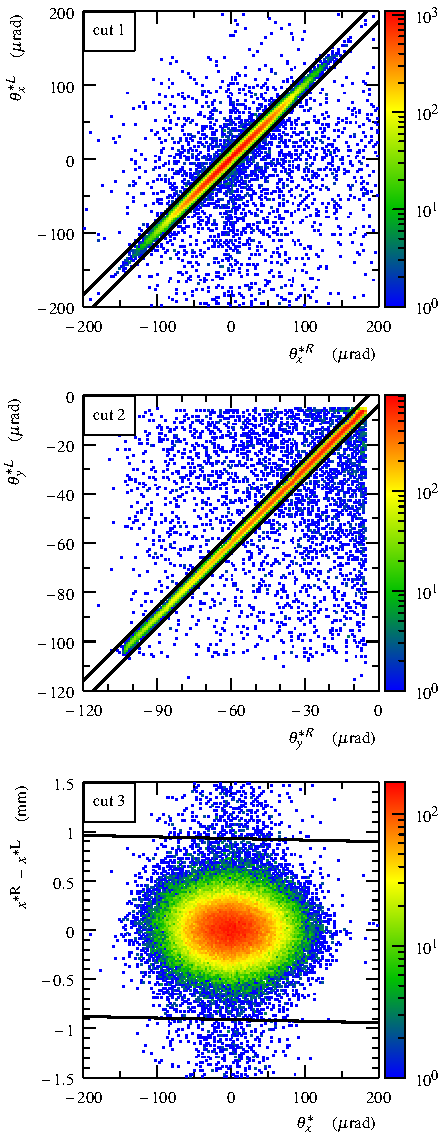
\includegraphics{fig/cuts.pdf}
\caption{%
Correlation plots for the event selection cuts presented in Table~\ref{tab:cuts}, showing events with diagonal topology 45 top -- 56 bottom. The solid black lines delimit the signal region within $\pm 4\un{\sigma}$.
}
\label{fig:cuts}
\end{center}
\end{figure}


%-------------------------

\subsubsection{Background}
\label{sec:background}

As the RPs were very close to the beam, one may expect an enhanced background from coincidence of beam halo protons hitting detectors in the two arms. Other background sources (pertinent to any elastic analysis) are: central diffraction and pile-up of two single diffraction events.

The background rate (i.e.~impurity of the elastic tagging) is studied by plotting the discriminators from Table~\ref{tab:cuts} under various cut combinations, see an example in Figure~\ref{fig:tag bckg}. While the central part (signal) remains essentially constant, the tails (background) are strongly suppressed when the number of cuts is increased. This interpretation is further supported by the discriminator distributions from non-diagonal RP track configurations (\textit{45 bottom -- 56 bottom} or \textit{45 top -- 56 top}), artificially treated like diagonal signatures by inverting the coordinate signs in the arm 45; see the dashed distributions in the figure. These non-diagonal configurations cannot contain any elastic signal and hence consist purely of background. Since in background events diagonal and non-diagonal signatures are equally frequent, the number of non-diagonal events surviving the cuts will be similar to the number of background events remaining in the diagonal signal region. The background is barely observable and one can estimate $1 - {\cal B} < 10^{-4}$.


\begin{figure}
\begin{center}
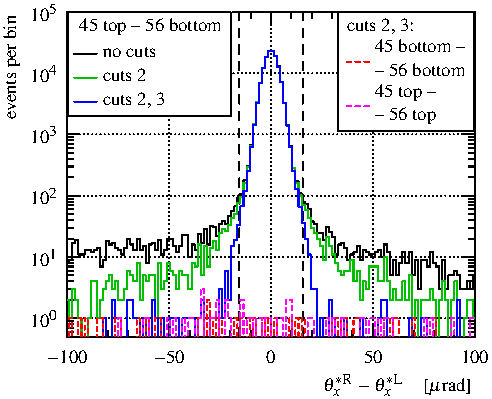
\includegraphics{fig/cut_distributions.pdf}
\caption{%
Distributions of discriminator 1, i.e. the difference between the horizontal scattering angle reconstructed from the right and the left arm. Solid curves: data from diagonal 45 top -- 56 bottom, the different colours correspond to various combinations of the selection cuts (see numbering in Table~\ref{tab:cuts}). Dashed curves: data from anti-diagonal RP configurations, obtained by inverting track coordinates in the left arm. The vertical dashed lines represent the boundaries of the signal region ($\pm 4\un{\sigma}$).
}
\label{fig:tag bckg}
\end{center}
\end{figure}

%-------------------------

\subsubsection{Acceptance Correction}
\label{sec:acc corr}

The acceptance of elastic protons is limited by two factors: sensor coverage (relevant for low $|\theta^*_y|$) and LHC beam aperture (at $|\theta^*_y| \approx 100\un{\mu rad}$). Moreover, there is a region in the kinematic parameter space where elastic protons may interact with the horizontal RPs leading to uncertain detection efficiency. To avoid this region, an additional fiducial cut has been adopted: $-50 < \theta_x^* < 80\un{\mu rad}$. In the far vertical RPs, this restriction corresponds to about $-2.3 < x < 3.7\un{mm}$. All acceptance related cuts are visualised in Figure~\ref{fig:acc corr princ}.

\begin{figure}
\begin{center}
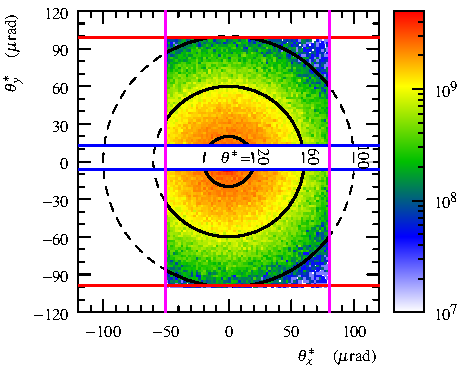
\includegraphics{fig/acc_corr_phi_lab.pdf}
\caption{%
Distribution of scattering angle projections $\theta_y^*$ vs.~$\theta_x^*$. The upper (lower) part comes from the diagonal 45 bottom -- 56 top (45 top -- 56 bottom). The red horizontal lines represent cuts due to the LHC apertures, the blue horizontal lines cuts due to the sensor edges. The vertical magenta lines delimit the fiducial region with detection efficiency not affected by the horizontal RPs. The dotted circles show contours of constant scattering angle $\theta^*$ as indicated in the middle of the plot (values in micro-radians). The parts of the contours within acceptance are emphasized in thick black.
}
\label{fig:acc corr princ}
\end{center}
\end{figure}

The correction for the above limitations includes two contributions -- a geometrical correction ${\cal A}_{\rm geom}$ reflecting the fraction of the phase space within the acceptance and a component ${\cal A}_{\rm fluct}$ correcting for fluctuations around the vertical acceptance limitations:
\begin{equation}
{\cal A}(\theta^*, \theta_y^*) = {\cal A}_{\rm geom}(\theta^*)\ {\cal A}_{\rm fluct}(\theta_y^*)\ .
\end{equation}
The fiducial cuts in $\theta_x^*$ have been been given sufficient margin from the region with uncertain efficiency to render the respective fluctuation correction negligible.

The calculation of the geometrical correction ${\cal A}_{\rm geom}$ is based on the azimuthal symmetry of elastic scattering, experimentally verified for the data within acceptance. As shown in Figure \ref{fig:acc corr princ}, for a given value of $\theta^*$ the correction is given by:
\begin{equation}
\label{eq:acc geom}
{\cal A_{\rm geom}}(\theta^*) = {
	\hbox{full arc length}\over 
	\hbox{arc length within acceptance}
} \ .
\end{equation}

The correction ${\cal A}_{\rm fluct}$ is calculated analytically from the probability that any of the two elastic protons leaves the region of acceptance due to the vertical beam divergence. The beam divergence distribution is modelled as a Gaussian with the spread determined by the method described in Section~\ref{sec:resolution}. This contribution is sizeable only close to the acceptance limitations. Data from regions with corrections larger than $2.5$ are discarded. The uncertainties are related to the resolution parameters. For the lowest $|t|$ bin their relative values are: vertical beam divergence: $2\un{\%}$, left-right asymmetry: $1\un{\%}$, and non-Gaussian shape: $1\un{\%}$.

Figure~\ref{fig:acc corr res} shows an example of the $t$-dependence of the acceptance correction for the diagonal reaching lower $|t|$-values. Since a single diagonal cannot cover more than half of the phase space, the minimum value of the correction is $2$. The very low $|t|$ data points with the full correction larger than $10$ are discarded to avoid biases. At the high-$|t|$ end all data points are kept.


\begin{figure}
\begin{center}
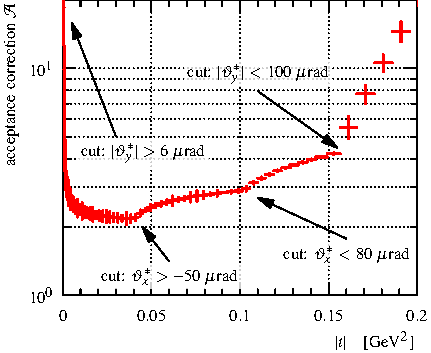
\includegraphics{fig/acc_corr_hist_lab.pdf}
\caption{%
Full acceptance correction, ${\cal A}$, for diagonal 45 bottom -- 56 top. The points give the mean value per bin, the error bars indicate the standard deviation. The abrupt changes in the shape correspond to acceptance cuts as indicated by the arrows.
}
\label{fig:acc corr res}
\end{center}
\end{figure}



%-------------------------

\subsubsection{Inefficiency Corrections}
\label{sec:ineff corr}

Since the overall normalisation will be determined from another dataset (see Section~\ref{sec:normalisation}), any inefficiency correction that does not alter the $t$-distribution shape does not need to be considered in this analysis (trigger, data acquisition and pile-up inefficiency discussed in~\cite{epl101-el,prl111}). The remaining inefficiencies are related to the inability of a RP to resolve the elastic proton track.

One such case is when a single RP does not detect and/or reconstruct a proton track, with no correlation to other RPs. This type of inefficiency, ${\cal I}_{3/4}$, is evaluated by removing the RP from the tagging cuts (Table \ref{tab:cuts}), repeating the event selection and calculating the fraction of recovered events. A typical example is given in Figure~\ref{fig:eff 3/4}, showing that the efficiency decreases gently with the vertical scattering angle. This dependence originates from the fact that protons with larger $|\theta_y^*|$ hit the RPs further from their edge and therefore the potentially created secondary particles have more chance to induce additional signal. Since the RP detectors can resolve only a single track, a secondary particle track prevents from using the affected RP in the analysis.

\begin{figure}
\begin{center}
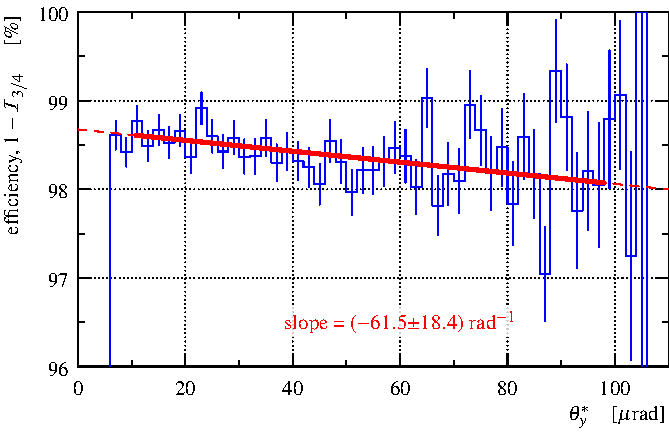
\includegraphics{fig/eff3outof4_fits.pdf}
\caption{%
Single-RP uncorrelated inefficiency for the near bottom RP in the right arm. The rapid drop at $\theta_y^* \approx 8\un{\mu rad}$ is due to acceptance effects at the sensor edge. The red lines represent a linear fit of the efficiency dependence on the vertical scattering angle (solid) and its extrapolation to the regions affected by acceptance effects (dashed).
}
\label{fig:eff 3/4}
\end{center}
\end{figure}

Another source of inefficiency are proton interactions in a near RP affecting simultaneously the far RP downstream. The contribution from these near-far correlated inefficiencies, ${\cal I}_{2/4}$, is determined by evaluating the rate of events with high track multiplicity ($\gtrsim$ 5) in both near and far RPs. Events with high track multiplicity simultaneously in a near top and near bottom RP are discarded as such a shower is likely to have started upstream from the RP station and thus be unrelated to the elastic proton interacting with detectors. The outcome, ${\cal I}_{2/4} \approx 1.5\un{\%}$, is compatible between left/right arms and top/bottom RP pairs and compares well to Monte-Carlo simulations (e.g.~section 7.5 in \cite{hubert-thesis}).

The full correction is calculated as
\begin{equation}
\label{efficiency}
	{\cal E}(\theta_y^*) = {1\over 1 - \left( \sum\limits_{i\in \rm RPs} {\cal I}^i_{3/4}(\theta_y^*) + 2 {\cal I}_{2/4} \right) } \ .
\end{equation}
The first term in the parentheses sums the contributions from the four RPs of a diagonal and increases from about $16$ to $18\un{\%}$ from the lowest to the highest $|\theta_y^*|$. These values are higher than in the previous analyses (e.g.~Section 5.2.4 in \cite{8tev-90m}) due the contribution from the far RPs in the left arm. The reconstruction efficiency in these pots is decreased by showers initiated by beam halo protons in the horizontal RPs upstream.

%The second term amounts to about $3\un{\%}$.

\iffalse
\> 3-out-of-4 results
\>> right arm: typical results (near $\approx 98\un{\%}$, far $\approx 96.5\un{\%}$ efficiency)
\>> left arm: efficiency in far RP unexpectedly low ($\approx 90\un{\%}$) -- due to showers in horizontal RPs (horizontal in left arm closer that in the right one) -- but experimentally determinable and thus fully correctable
\fi



%-------------------------

\subsubsection{Unfolding of Resolution Effects}
\label{sec:unfolding}

Due to the very small beam divergence, the correction for resolution effects can be safely determined by the following iterative procedure. The differential cross-section data are fitted by a smooth curve which serves as an input to a numerical-integration calculation of the smeared $t$-distribution (using the resolution parameters determined in Section~\ref{sec:resolution}). The ratio between the smeared and the non-smeared $t$-distributions gives a set of per-bin correction factors. Applying them to the yet uncorrected differential cross-section yields a better estimate of the true $t$-distribution, which can be used as input to the next iteration. The iteration stops when the difference between the input and output $t$-distributions becomes negligible, which is typically achieved after the second iteration. The final correction is negligible (${\cal U} \approx 1$) for all bins except at very low $|t|$ where the rapid cross-section growth occurs, see Figure~\ref{fig:unfolding}.

For the uncertainty estimate, the uncertainties of the $\theta_x^*$ and $\theta_y^*$ resolutions (accommodating the full time variation) as well as fit-model dependence have been considered, each contribution giving a few per-mille for the lowest-$|t|$ bin.

\begin{figure}
\begin{center}
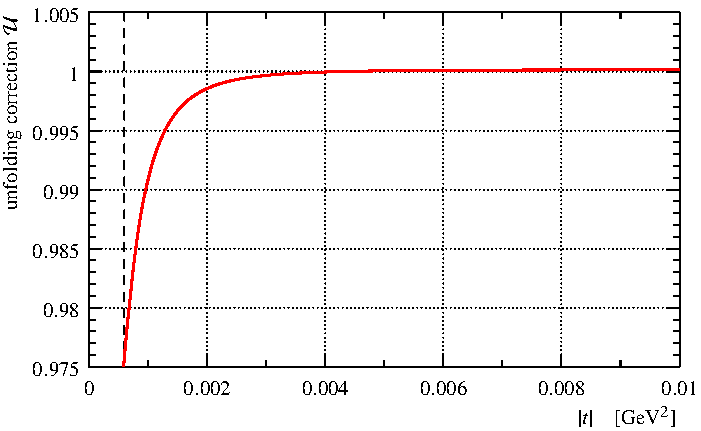
\includegraphics{fig/unfolding.pdf}
\caption{%
Unfolding correction for the close diagonal (45 bottom -- 56 top). The vertical dashed line indicates the position of the acceptance cut due to sensor edges.
}
\label{fig:unfolding}
\end{center}
\end{figure}

%-------------------------

\subsubsection{Normalisation}
\label{sec:normalisation}

The normalisation ${\cal N}$ is determined by requiring the same cross-section integral between $|t| = 0.014$ and $0.203\un{GeV^2}$ as for dataset 1 published in \cite{prl111}, where a luminosity-independent calibration was applied. The leading uncertainty of the scaling factor $4.2\un{\%}$ comes from the luminosity-independent method.
% transfer negligible ($0.5\un{\%}$).
% stat: 0.3%, syst: 0.3% (DS2 at 90m), 0.3% (1km)


%-------------------------

\subsubsection{Binning}
\label{sec:binning}

At very low $|t|$, where the cross-section varies the fastest ($\approx 0.001\un{GeV^2}$), a fine binning is used. In the middle of the $|t|$ range ($\approx 0.03\un{GeV^2}$), the bin width is chosen to give about $1\un{\%}$ statistical uncertainty. This rule is abandoned at higher $|t|$ (above $0.07\un{GeV^2}$) in favour of bins with a constant width of $0.01\un{GeV^2}$ to avoid excessively large bins.


%-------------------------

\subsubsection{Systematic Uncertainties}
\label{sec:systematics}

Besides the systematic uncertainties mentioned at the above analysis steps, the beam momentum uncertainty of $0.1\un{\%}$ (cf.~Section 5.2.8 in \cite{8tev-90m}) needs to be considered when the scattering angles are translated to $t$, see Eq.~(\ref{eq:th t}).

Two different methods are used to propagate the systematic effects into the $t$-distribution. The first is based on a Monte-Carlo simulation which uses a fit of the final differential cross-section data to generate the true $t$-distribution. In parallel, another $t$-distribution is built, introducing one of the above mentioned systematic effects at $1\un{\sigma}$ level. The difference between the two $t$-distributions gives the systematic effect on the differential cross-section. The second method is similar, however using numerical integration techniques instead of Monte-Carlo simulations. Both methods are formally equivalent to evaluating
\begin{equation}
\label{eq:syst mode}
\delta s_{q}(t) \equiv \frac{\partial(\d\sigma/\d t)}{\partial q}\ \delta q\ ,
\end{equation}
where $\delta q$ corresponds to a $1\un{\sigma}$ bias in the quantity $q$ responsible for a given systematic effect.

The Monte-Carlo simulations show that the combined effect of several systematic errors is well approximated by linear combination of the individual contributions from Eq.~(\ref{eq:syst mode}).


%----------------------------------------------------------------------------------------------------

\subsection{Systematic Cross-Checks}
\label{sec:cross checks}

Compatible results have been obtained by analysing data subsets of events from different bunches, different diagonals and different time periods -- in particular those right after and right before the beam cleanings.



 %----------------------------------------------------------------------------------------------------
\subsection{Final Data Merging}
\label{sec:final data merging}

Finally, the differential cross-section histograms from both diagonals are merged. This is accomplished by a per-bin weighted average, with the weight given by inverse squared statistical uncertainty. The statistical and systematic uncertainties are propagated accordingly. For the systematic ones, the correlation between the diagonals is taken into account. For example the vertical (mis-)alignment of the RPs of one unit is almost fully correlated; thus the effect on the differential cross-section is opposite for the two diagonals and consequently its impact is strongly reduced once the diagonals are merged.

The cross-section values can be found in Table~\ref{tab:data} and visualised in Figure~\ref{fig:dsdt}. The figure clearly shows a rapid cross-section rise below $|t| \lesssim 0.002\un{GeV^2}$, which will later be interpreted as an effect due to electromagnetic interaction.

\input data_table.tex

\begin{figure*}
\vskip-5mm
\begin{center}
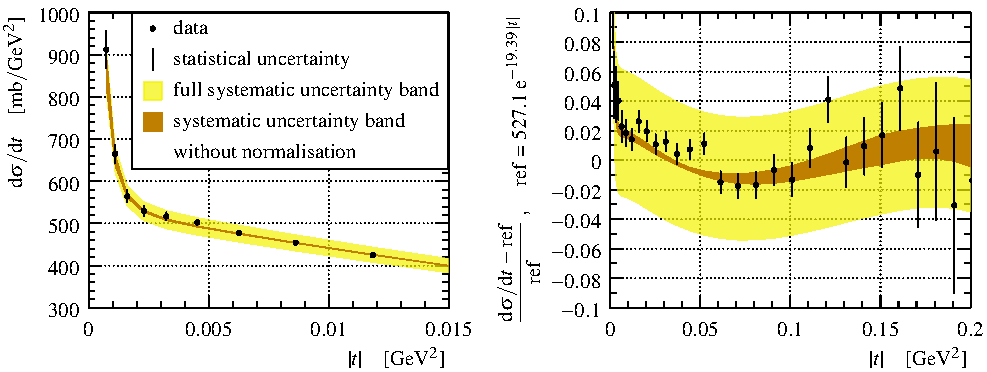
\includegraphics{fig/t_dist_tabulation.pdf}
\vskip-3mm
\caption{%
Differential cross-section from Table \ref{tab:data} with statistical (bars) and systematic uncertainties (bands). The yellow band represents all systematic uncertainties, the brown one all but normalisation. The bands are centred around a data fit including both nuclear and Coulomb components (Eqs.~(\ref{eq:int kl}), (\ref{eq:nuc phase con}) and (\ref{eq:nuc mod}) with $N_b=3$). INSET: a low-$|t|$ zoom featuring cross-section rise due to the Coulomb interaction.
}
\label{fig:dsdt}
\end{center}
\end{figure*}

The final systematic uncertainties, except the $4.2\un{\%}$ coming from the normalisation, are summarised in Figure~\ref{fig:syst unc} where their impact on the differential cross-section is shown. The leading uncertainties include normalisation, optics imperfections, beam momentum offset and residual misalignment. The vertical misalignment is the dominant systematic effect in the very-low $|t|$ region. The leading effects are quantified in Table~\ref{tab:data} and can be used to approximate the covariance matrix of systematic uncertainties:
\begin{equation}
\label{eq:covar mat}
\mat V_{ij} = \sum_{q} \delta s_{q}(i)\ \delta s_{q}(j)\: ,
\end{equation}
where $i$ and $j$ are bin indices (row numbers in Table~\ref{tab:data}) and the sum goes over the leading error contributions $q$ (six right-most columns in the table).



\begin{figure*}
\begin{center}
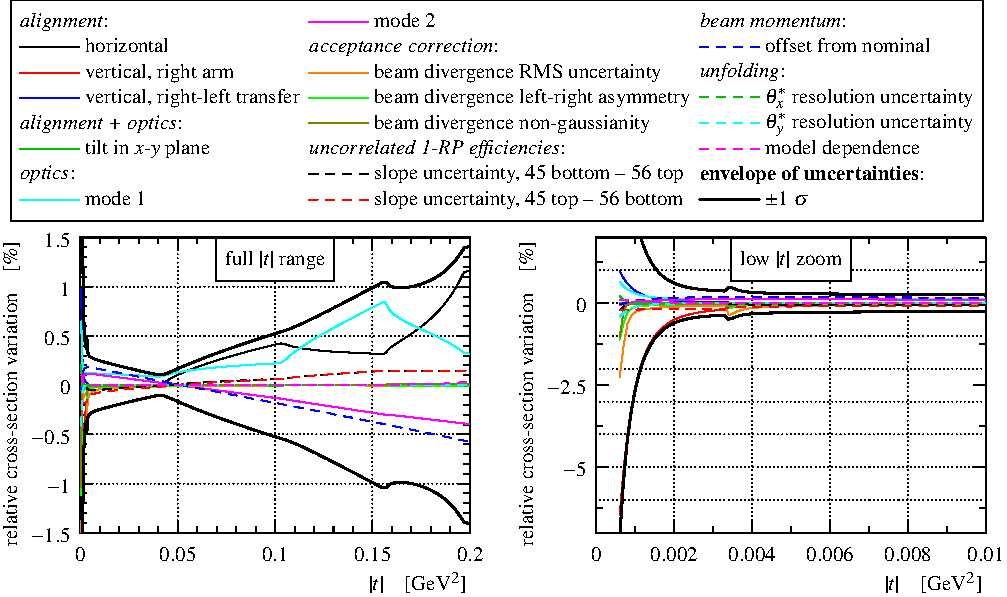
\includegraphics{fig/systematic_uncertainties.pdf}
\caption{%
Impact of $t$-dependent systematic effects on the differential cross-section. Each curve corresponds to a systematic error of $1\un{\sigma}$, cf.~Eq.~(\ref{eq:syst mode}). The two contributions due to the optics correspond to the two vectors in Eq.~(\ref{eq:opt bias modes}). The envelope is determined by summing all shown contributions in quadrature for each $|t|$ value.
}
\label{fig:syst unc}
\end{center}
\end{figure*}
